\documentclass[12pt]{report}
\usepackage{amssymb}
\usepackage{amsmath}

\usepackage{multicol}
\usepackage{graphicx}
\usepackage{subfigure}
\usepackage{verbatim}

%\usepackage{adjustbox}

\usepackage[letterpaper,left=1cm,right=2cm, top=1.5cm,
bottom=1.5cm,head=0cm,foot=1cm]{geometry}

\parindent=0in


\newcommand{\m}{\mbox{ m }}
\newcommand{\kg}{\mbox{ kg }}
\newcommand{\s}{\mbox{ s }}
\newcommand{\ke}{\mbox{\small KE}}
\newcommand{\pe}{\mbox{\small PE}}


\newcommand{ \probDir}[1]{{ \bf\small #1 \mbox{  }}}

\newcommand{ \breakList}{\setcounter{saveenum}{\value{enumi}} \end{enumerate}}
\newcommand{ \contList}{\begin{enumerate} \setcounter{enumi}{\value{saveenum}}}

\newcounter{saveenum}

\def \wspace{5cm}

%%%%%%%%%%%%%%%%%%%%%%%%%%%%%%%%%%%%%%%%%
\begin{document}

{\bf{Honors Physics} \hfill Notepage: The net force, and Newton's $2^{\mbox{\tiny nd}}$ \hfill {Mr. Kelley}} \\ \\
%%%%%%%%%%

\vspace{1cm}

\hfill \parbox{6cm}{\centering Sometimes there are many \\ forces acting on a body.} \raisebox{-2cm}{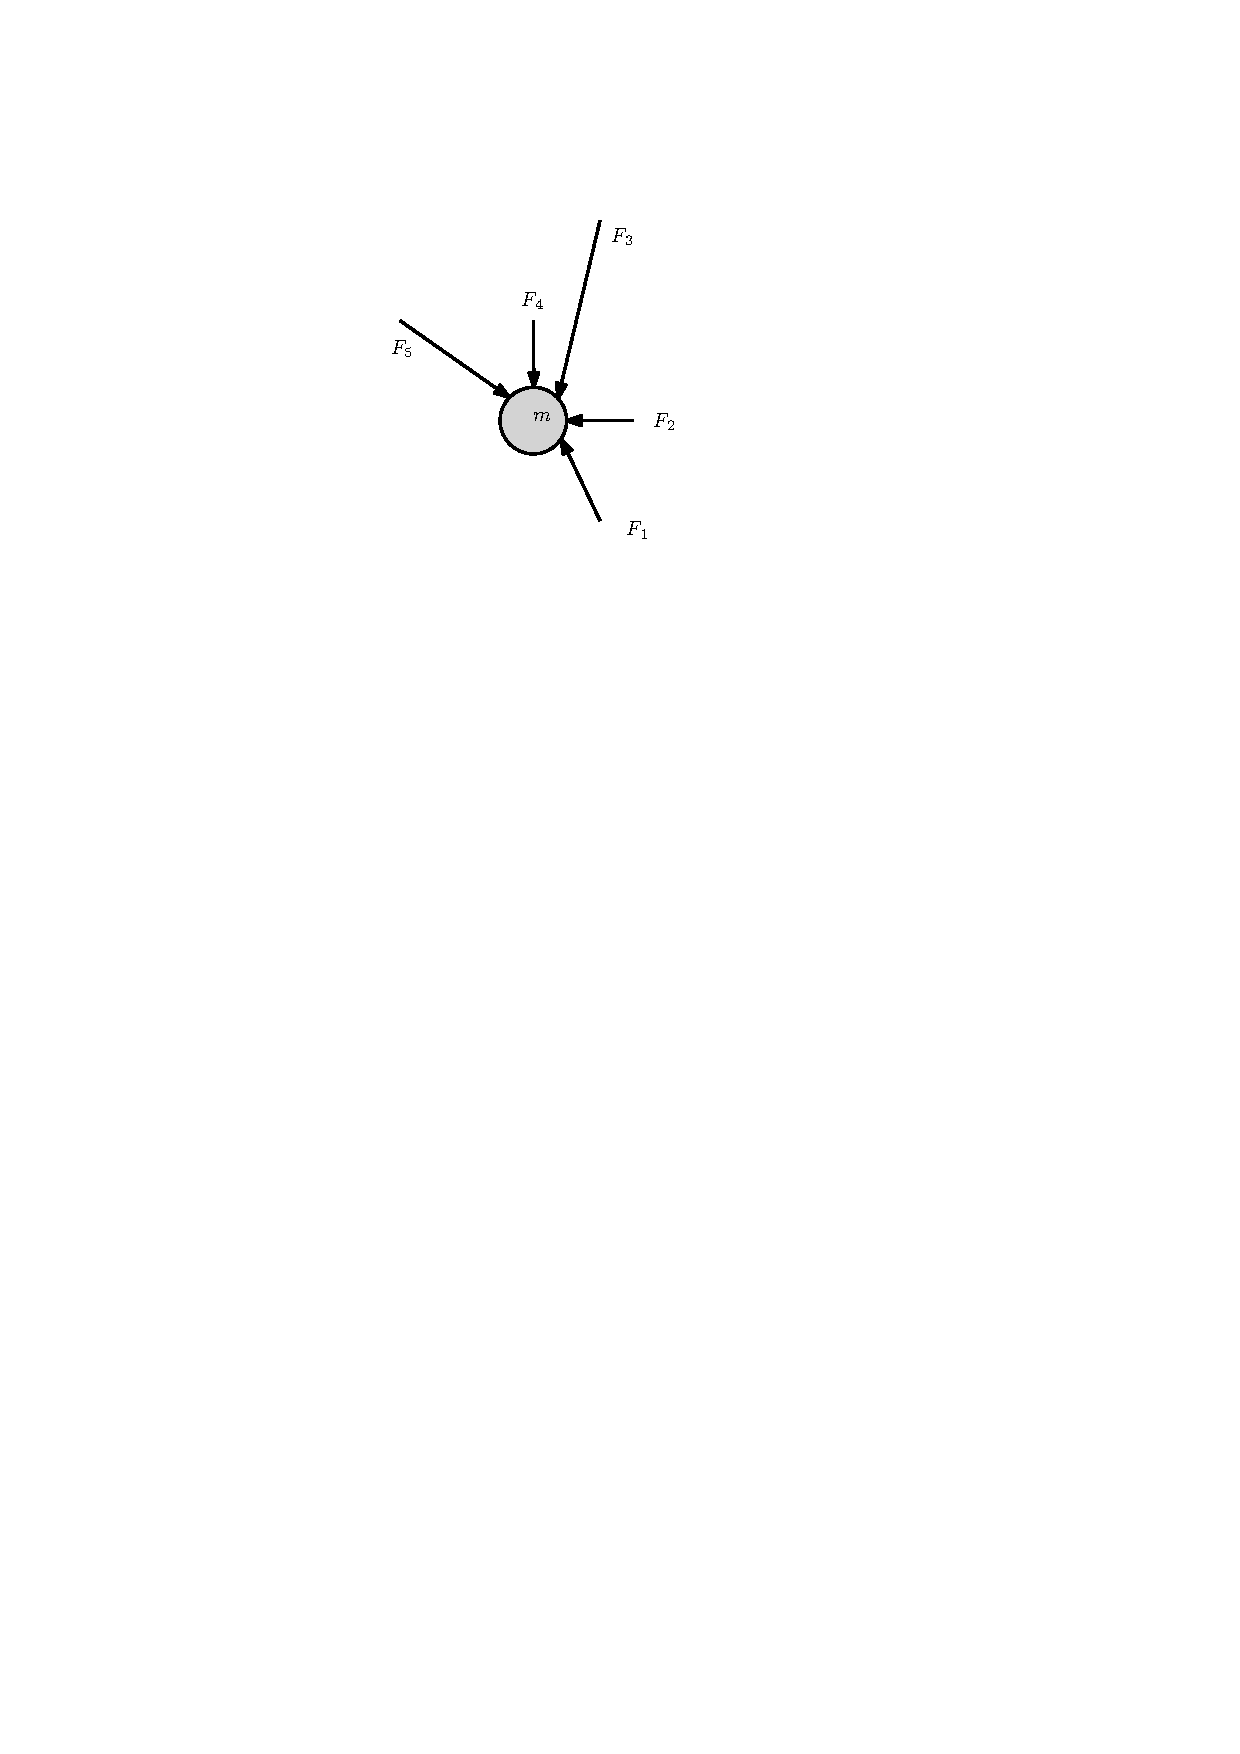
\includegraphics{sumForces_1}} \hspace{5cm}

\vspace{1.5cm}

\hspace{5cm} \raisebox{-5.5cm}{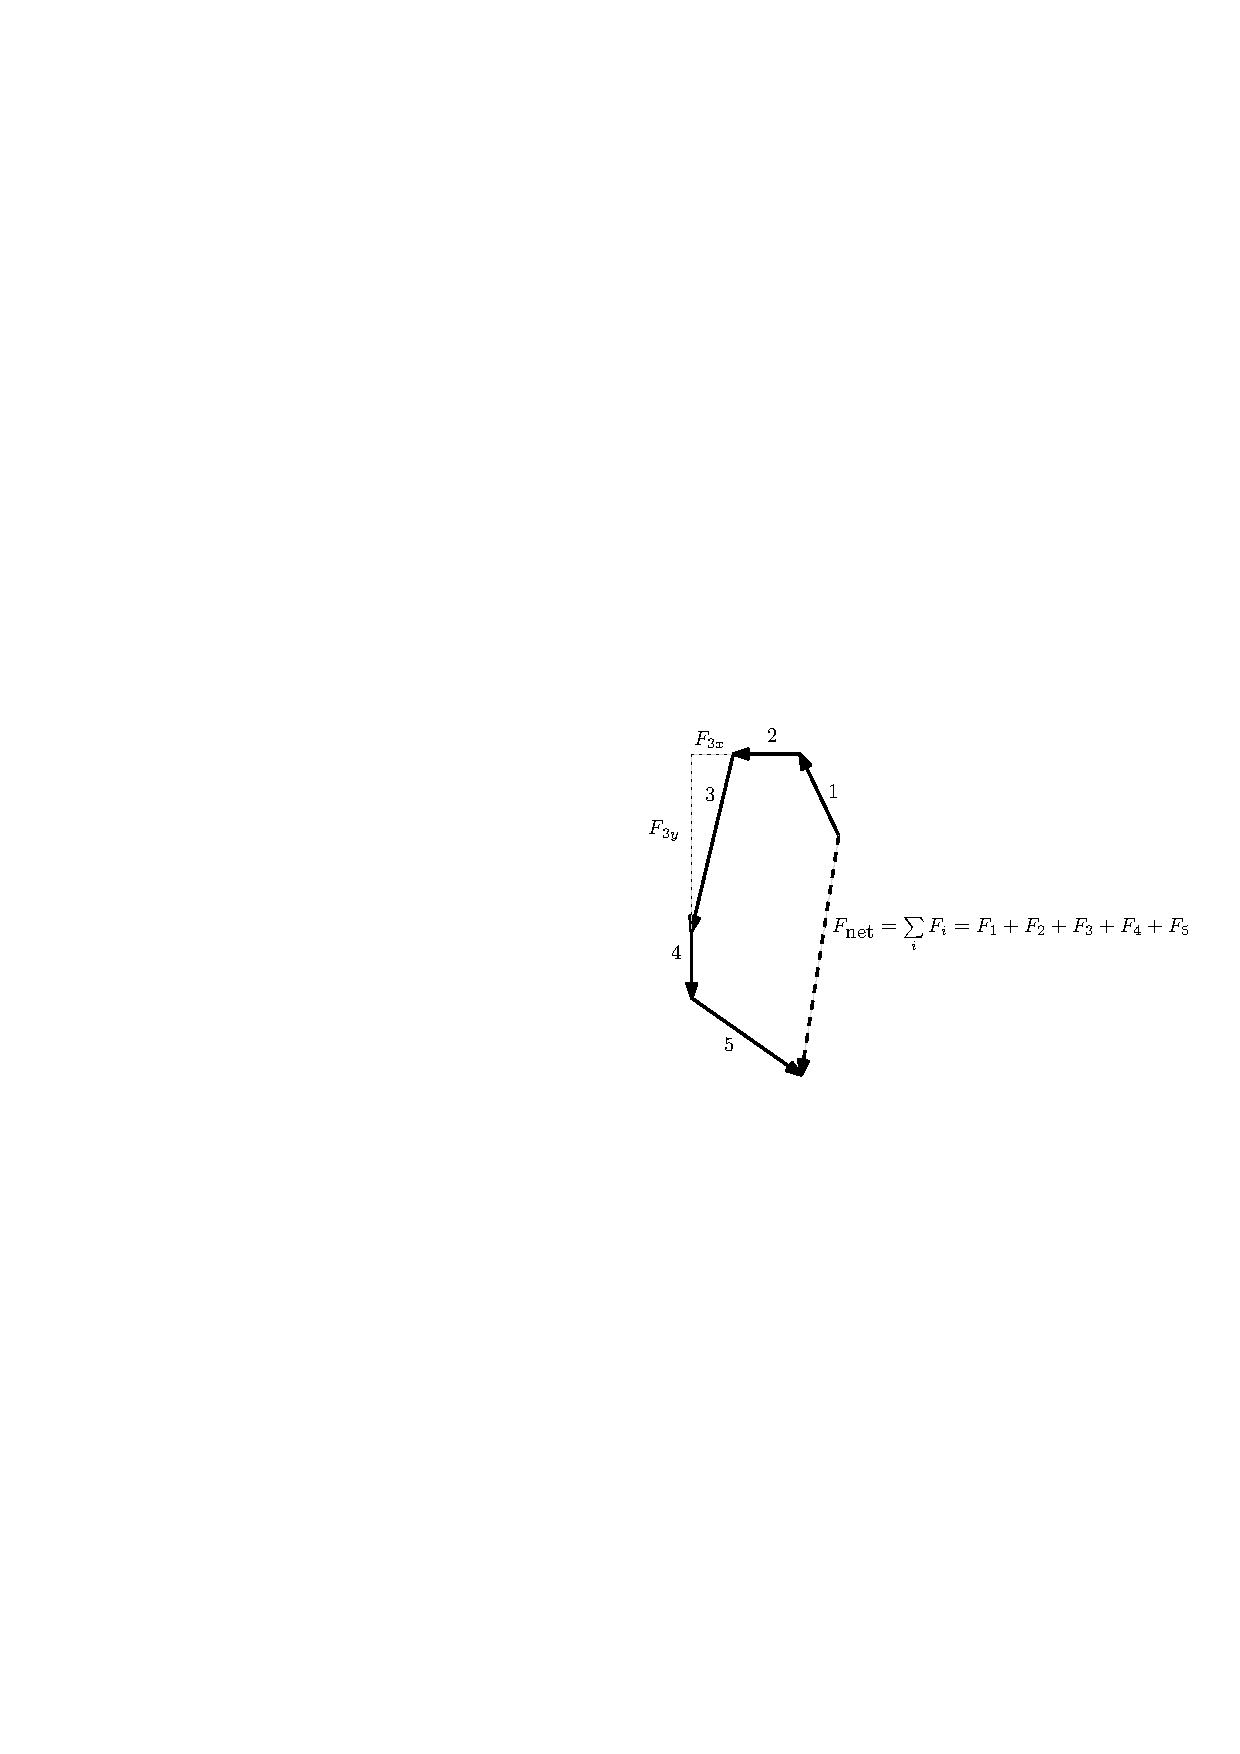
\includegraphics{sumForces_2}} \hspace{-5cm} \parbox{6.5cm}{To find the net force, we find the sum of the forces using vector addition.  Think of this like counting on a number line in two dimensions; rise over run.  When you take the sine, you get the $y$-component or rise.  When you take the cosine, you get the $x$-component or run.}

\hfill \parbox{6cm}{Whatever the net force is, \emph{that} is used to understand the acceleration of an object.  If you already know the acceleration of an object, then you can say something about the net force acting on it.} \raisebox{-2cm}{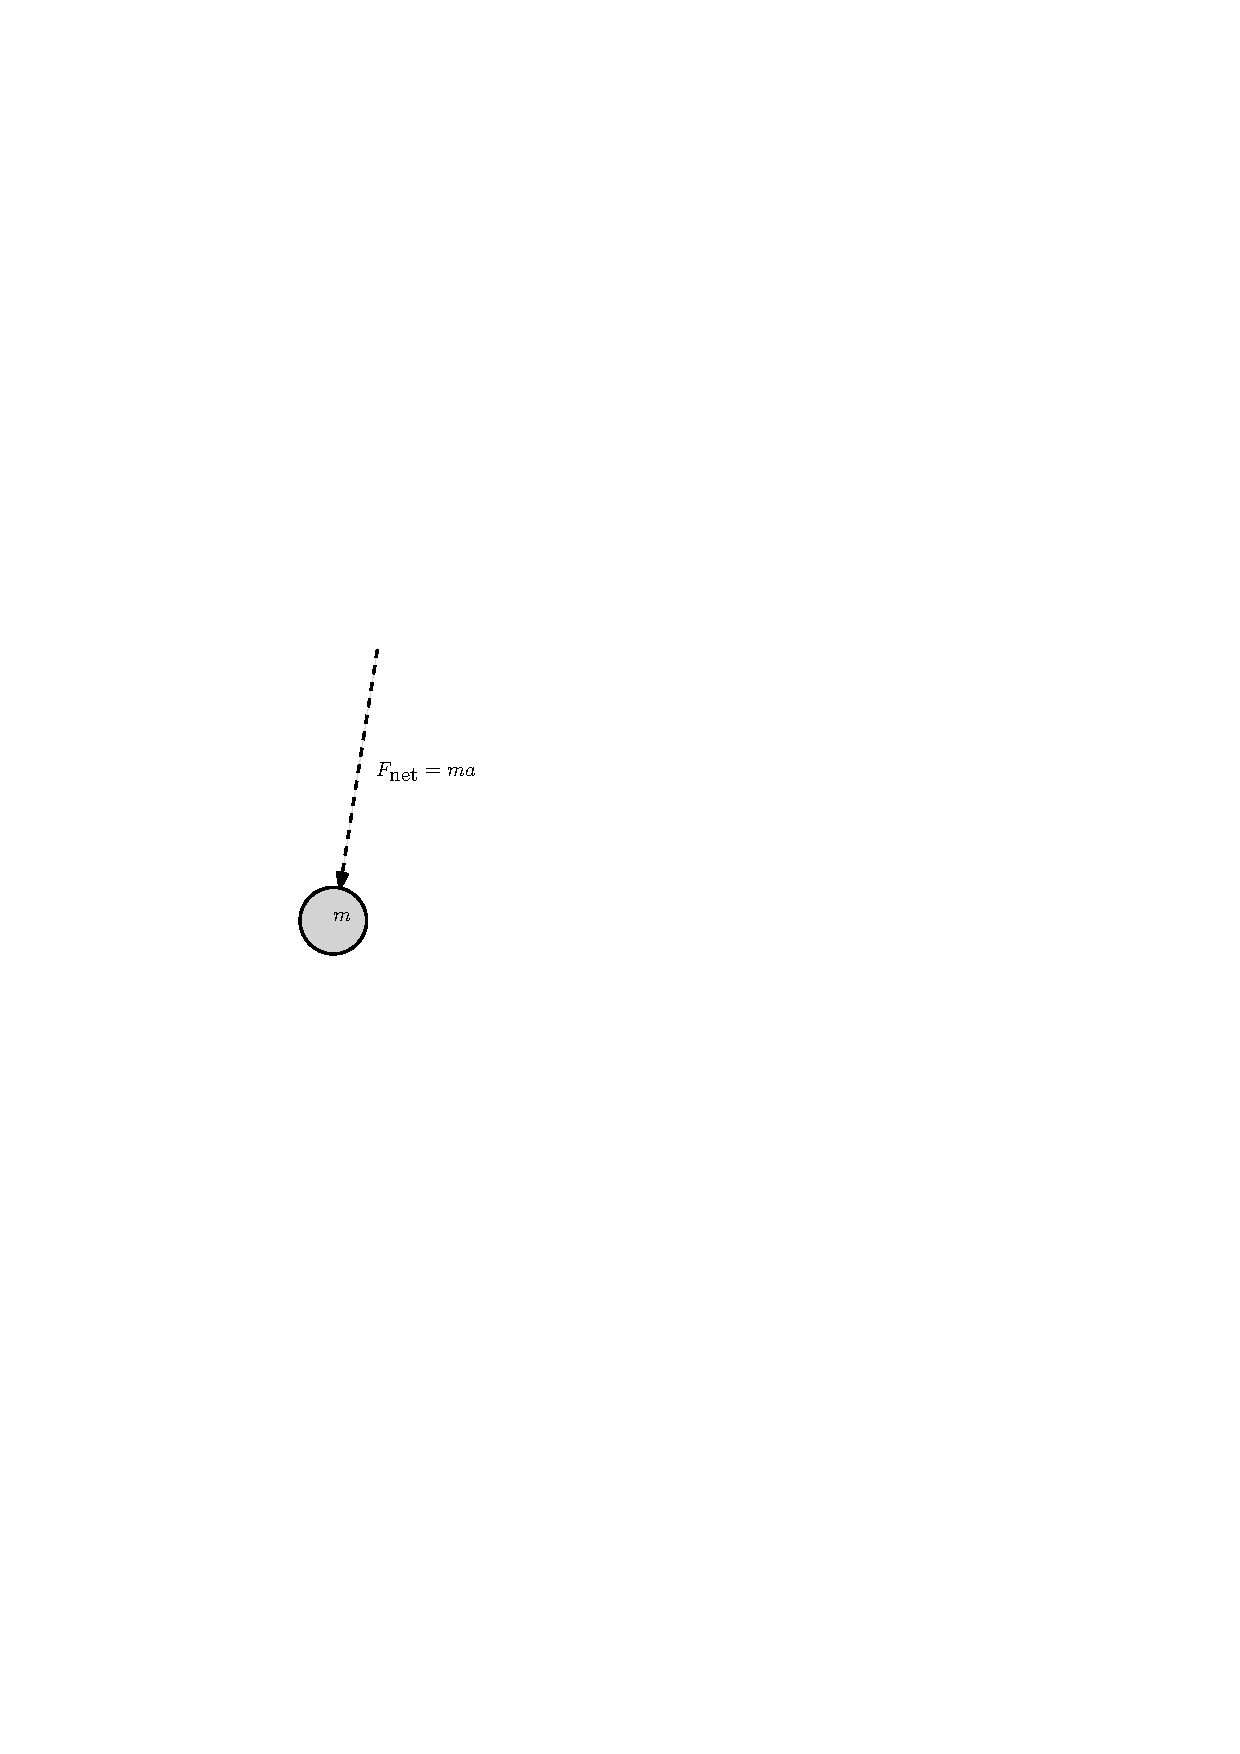
\includegraphics{sumForces_3}}  \hspace{7cm}

\end{document}